\documentclass[11pt]{article}
\usepackage{fullpage}
\usepackage{graphicx}
\usepackage{tikz}
\usepackage{hyperref}

\title{CS63 Spring 2017\\Lab 7: Neural Networks}
\author{David Chang and Won Chung}%TODO: replace \ldots with your names

\begin{document}

\maketitle

\section{XOR}

With random seed 10 %TODO: replace \ldots with your seed
our network achieved 100\% accuracy on the XOR data set after 1470 %TODO: replace ldots with epochs
training epochs.
The resulting neural network is shown in the following diagram.

%TODO: fill in the weights with ONE DECIMAL DIGIT of precision
\begin{center}
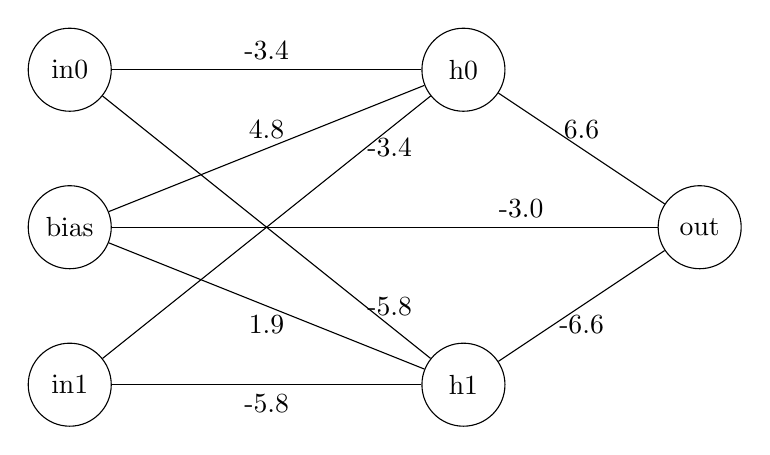
\begin{tikzpicture}
\tikzstyle{neuron}=[draw, circle, minimum size=30pt]

\draw (0,2) node[neuron] (bias) {bias};
\draw (0,4) node[neuron] (in0) {in0};
\draw (0,0) node[neuron] (in1) {in1};
\draw (5,4) node[neuron] (h0) {h0};
\draw (5,0) node[neuron] (h1) {h1};
\draw (8,2) node[neuron] (out) {out};

\draw (in0) edge node[above] {-3.4} (h0);
\draw (in0) edge node[very near end, above] {-5.8} (h1);
\draw (in1) edge node[very near end, below] {-3.4} (h0);
\draw (in1) edge node[below] {-5.8} (h1);
\draw (h0) edge node[above] {6.6} (out);
\draw (h1) edge node[below] {-6.6} (out);
\draw (bias) edge node[above] {4.8} (h0);
\draw (bias) edge node[below] {1.9} (h1);
\draw (bias) edge node[near end, above] {-3.0} (out);
\end{tikzpicture}
\end{center}


%TODO: Explain how the network solved the XOR problem based on these parameters.
%Hint: describe what boolean function (logic gate) each node is approximating.
By creating truth tables for h0 and h1 as a function of the two inputs plus the bias, the boolean
functions of each node can be approximated. If the weighted sum of the inputs is greater than 0, the
boolean output is 1 and if the weigthed sum of the inputs is less than 0, the boolean output is 0. h0
has the truth table of a NAND gate, and h1 has the truth table of a NOR gate so these two can be
approximated as so. The out node as a function of h0 and h1 and the bias has a truth table of h0 AND NOT
h1 so that can be approximated as such. This combination of boolean functions can be abstracted to be
simply an XOR gate.

\section{Keras}

Here is how we achieved 97.88{\%} %TODO: replace \ldots with test set accuracy
accuracy on the MNIST handwritten digit data set.

\subsection{Parameters}

\ldots
%TODO: describe the parameter settings you used
%Here's an example of a bulleted list:
%\begin{itemize}
%  \item One entry in the list
%  \item Another entry in the list
%\end{itemize}
\begin{itemize}
 \item activation='selu'
 \item activation='softmax'
 \item optimizer="Adadelta"
 \item loss="categorical$\_$crossentropy"
\end{itemize}

\subsection{Process}
%TODO: describe how you found the parameters above.
%If you found them online, be sure to provide a link with \url{ }
We founded and decided to use 'selu' and 'softmax' after combinations of activations. Then we found this link http://www.python36.com/mnist-handwritten-digits-classification-using-keras/ .
The link had 'Adadelta' as the optimizer and "categorical$\_$crossentropy" as the loss.
\subsection{Explanation}
%TODO: explain why the parameters you found are more successful than the default parameters.
The default parameters were the following:
\begin{itemize}
 \item activation='sigmoid'
 \item activation='sigmoid'
 \item optimizer="SGD"
 \item loss="mean$\_$squared$\_$error"
\end{itemize}

\noindent
SELU is f(x) = x $\cdot$ sigmoid(x) . Sigmoid has the weakness of the function being flat beoynd the -3 and +3 regions, meaning the gradients become small and approaching zero; the network is not learning well. SELU induces self-normalizing properties and converge the layers towards zero mean and unit variance, allowing for training a network with many layers. Since the gradients are vanishing for sigmoid and not for SELU, SELU is better. 

\noindent
Softmax is a type of sigmoid function, but is designed to handle multiple classes (sigmoid is designed to handle two cases). Softmax gives the probability of the input being in a specific class. Since there are many numbers, softmax is better than sigmoid in classification.

\noindent
The main difference between SGD and Adadelta is the learning rate. For SGD, if the learning rate is small, convergence is small. If the learning rate is large, it will lead to divergence. And the gradient of the loss changes after each iteration because of the variations in the training. Adadelta uses a decaying learning rate, restricting the size of accumulated past gradients. Adadelta is better since its convergence is based on the initial learning rate (i.e. convergence is ok even when the learning rate is large).

\noindent
Mean Squared Error has a too much emphasis on incorrect outputs. Using mean squared error also has the disadvantage the condition if the adjustment factor gets smaller, the change in weights get smaller and stall out the training. Categorical Cross Entropy takes into account the closeness of the prediction. Categorical Cross Entropy doesn't have the problem of the weight changes not becoming smaller and smaller leading to the training being stalled out.


\end{document}
